\noindent
The healthcare systems of the future will be highly decentralised, integrating home-, work- and environment-based monitoring into the hospital diagnostic systems, thus reducing costs and travel-associated risks while allowing patients to get faster diagnostics and better medical treatment (Figure~\ref{fig:dataExch}). As a consequence, medical data will need to be collected from a variety of sources and exchanged in a variety of ways, including over public networks that cannot be implicitly trusted. At the same time, we have more and more strict regulations about ownership and access rights for the patient data. Trans-national standards for data protection, such as the EU General Data Protection Regulation (GDPR)~\cite{gdpr}, will need to be combined with local regulations, giving very strict rules about who is allowed to access what part of patient data. Complying with these rules while, at the same time, facilitating data exchange and analytics in a decentralised way will be the main challenge for the future healthcare systems.

\begin{figure}[t!]
    \centering
    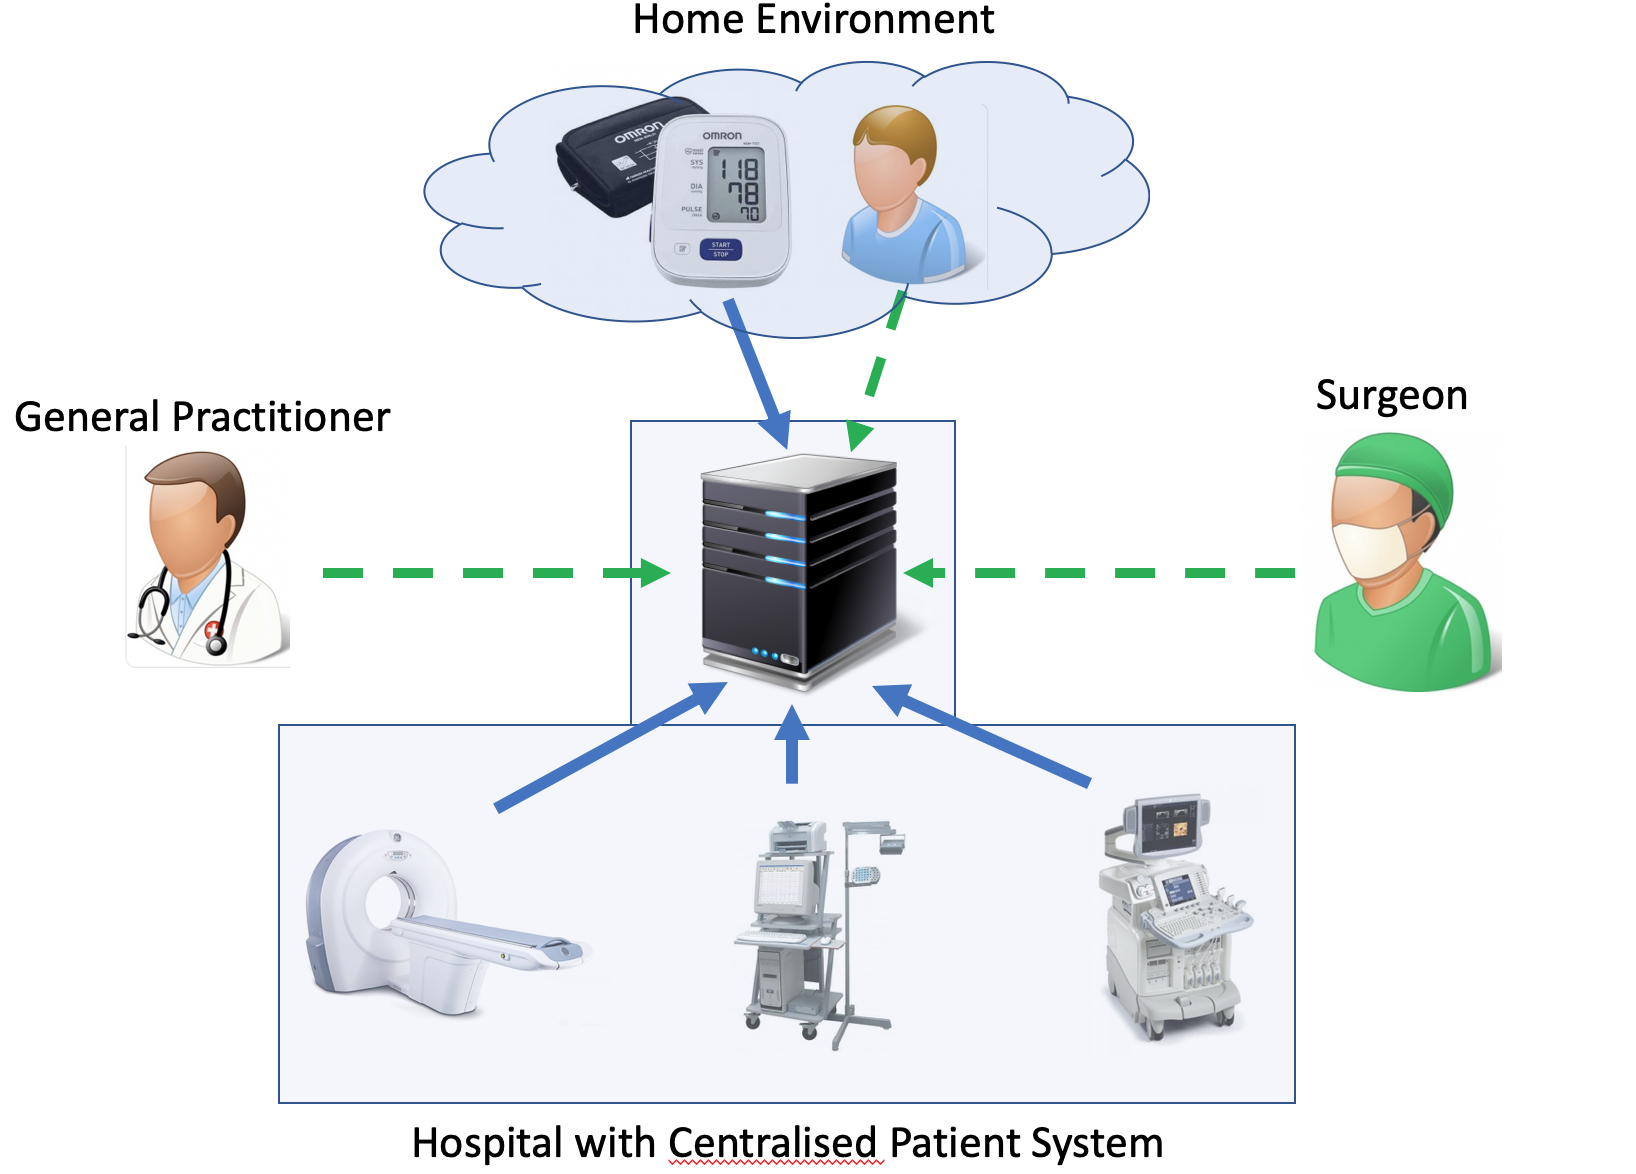
\includegraphics[width=70mm]{images/DataExchange.png}
    \caption{Data Exchange in Modern Healthcare Systems}
    \label{fig:dataExch}
\end{figure}

In this paper, we describe a methodology that will be developed over the course of the ongoing \emph{Serums: Securing Medical Data in Smart Patient-Centric Healthcare Systems} EU H2020 project and that will address the issues of safe, secure and privacy-preserving storage, access, communication and analysis of the medical data in future-generation smart health centres. Our main goal is to put patients at the centre of the future healthcare provision in Europe, enhancing their personal care and maximising the quality of treatment that they will receive, while securing trust in the security and privacy of their confidential medical data. To this end, we aim to develop a complete tool-chain that will ensure security and privacy of data over its lifetime, from collection and storage to the distributed analytics.

To reduce the scope of the paper, we restrict our attention to a subset of the \emph{Serums} technologies. We propose a universal format for patient records, the aim of which is to allow uniform representation of patient data across different use cases, and describe its implementation using the \emph{data vault} concept from data science. We also describe \emph{FlexiPass}, an authentication mechanisms to access these records, together with the application of blockchain technology to control permissions, ensure only the allowed agents are allowed to access the relevant parts of patient records stored and processed within a \emph{data lake} and to save the record access history. We then describe a novel, \emph{privacy-preserving} data analytics mechanism which ensures that the analytics model does not accidentally leak any sensitive information. Finally, we present the \emph{data fabrication} methodology that allows generation, based on strict format of the smart patient records and rules for dependencies between its elements, synthetic but realistic data that will be used for rapid development and stress-testing of the \emph{Serums} technologies.


This paper makes the following concrete research contributions: 
\begin{itemize}
    \item We propose a \emph{Serums} methodology, with the associated interoperable tool-chain for management and analytics of confidential medical data in modern distributed healthcare systems;
    \item We describe initial implementations of the tools from the \emph{Serums} tool-chain;
    \item We evaluate the \emph{Serums} tool-chain on \emph{Edinburgh Cancer Gateway}, a real-world use case for predicting toxicity levels of cancer treatments. 
\end{itemize}


\section{Background}

\noindent
The emergence of Internet-of-Things (IoT) technology is having a profound effect on the development of modern healthcare systems. Traditionally, these systems have been highly centralised, with all of the health data relevant to a single patient residing in a central location within a hospital or health center, and all the measurement devices that were used to obtain this data (blood pressure monitors, CT scanners etc.) also residing within the same administrative unit. From the security and privacy point of view, collecting, storing and processing this data was relatively simple, since the data needed to be communicated over trusted networks. However, as personal medical devices become cheaper and more prevalent, it became clear that integrating home-based healthcare, with all of its advantages such as wearable devices with home monitoring sensors, into the holistic diagnostics and treatment plan for patients can significantly reduce cost and travel-associated risks while increasing the quality of healthcare provision. This, however, involves sharing of the private and confidential data across public networks, posing significantly more risk than when the data is only exchanged within a single trusted organisation. This scenario also presents a number of additional issues that need to be dealt with:
\begin{itemize}
    \item \emph{Ensuring Trust}. The patients must have a high degree of trust both that the smart healthcare system operates as intended, and that their privacy is fully protected.
    \item \emph{Security, Privacy and Anonymity}. The smart healthcare system must work efficiently as a whole in order to maximise the quality of patient care, yet must simultaneously provide high levels of security and support high expectations of privacy and anonymity.
    \item \emph{Control of the data}. The patients must have full control of their data, as required by the GDPR and other legislations, yet the data must be provided in a timely fashion to medical practitioners and specialists.
    \item \emph{Compliance to regulations.} In order to support emergency medicine or other forms of trans-border medical treatment, the smart healthcare system must comply with with multiple, possibly conflicting, legislative frameworks.
\end{itemize}

\subsection{The Serums Project}

\noindent
\emph{Serums: Securing Medical Data in Smart Patient-Centric Healthcare Systems} is a recently-started €4.47 M EU H2020 project that aims to produce tools and techniques for safe and secure collection, storage, communication and processing of health data. It includes three universities (University of St Andrews from Scotland, University of Cyprus and Universite Catholique de Louvain from Belgium), four industrial technology providers (IBM Science and Technology from Israel, Sopra Steria from the UK, Software Competence Center Hagenberg from Austria and Accenture BV from Netherlands) and two end-user healthcare centers (Zuyderland Medisch Centrum from Netherlands and Fundacio Clinic per a la Recerce Biomedica from Spain). The goal of the project is to provide technologies for
\begin{itemize}
    \item Security and protection of the shared medical data across untrusted networks;
    \item Integrating personal medical data, coming from various sources, into coherent and structured smart patient records;
    \item Data analytics techniques that will be able to deal with distributed data that cannot be moved to a central location;
    \item Authentication and trust mechanisms that will ensure that only properly authorised agents have access to the required part of personal and medical data;
    \item World-leading levels of compliance to the existing and emerging legal and ethical standards.
\end{itemize}

\section{Serums Tool-Chain For Smart Health Centre Systems}

\begin{figure}[ht!]
    \centering
    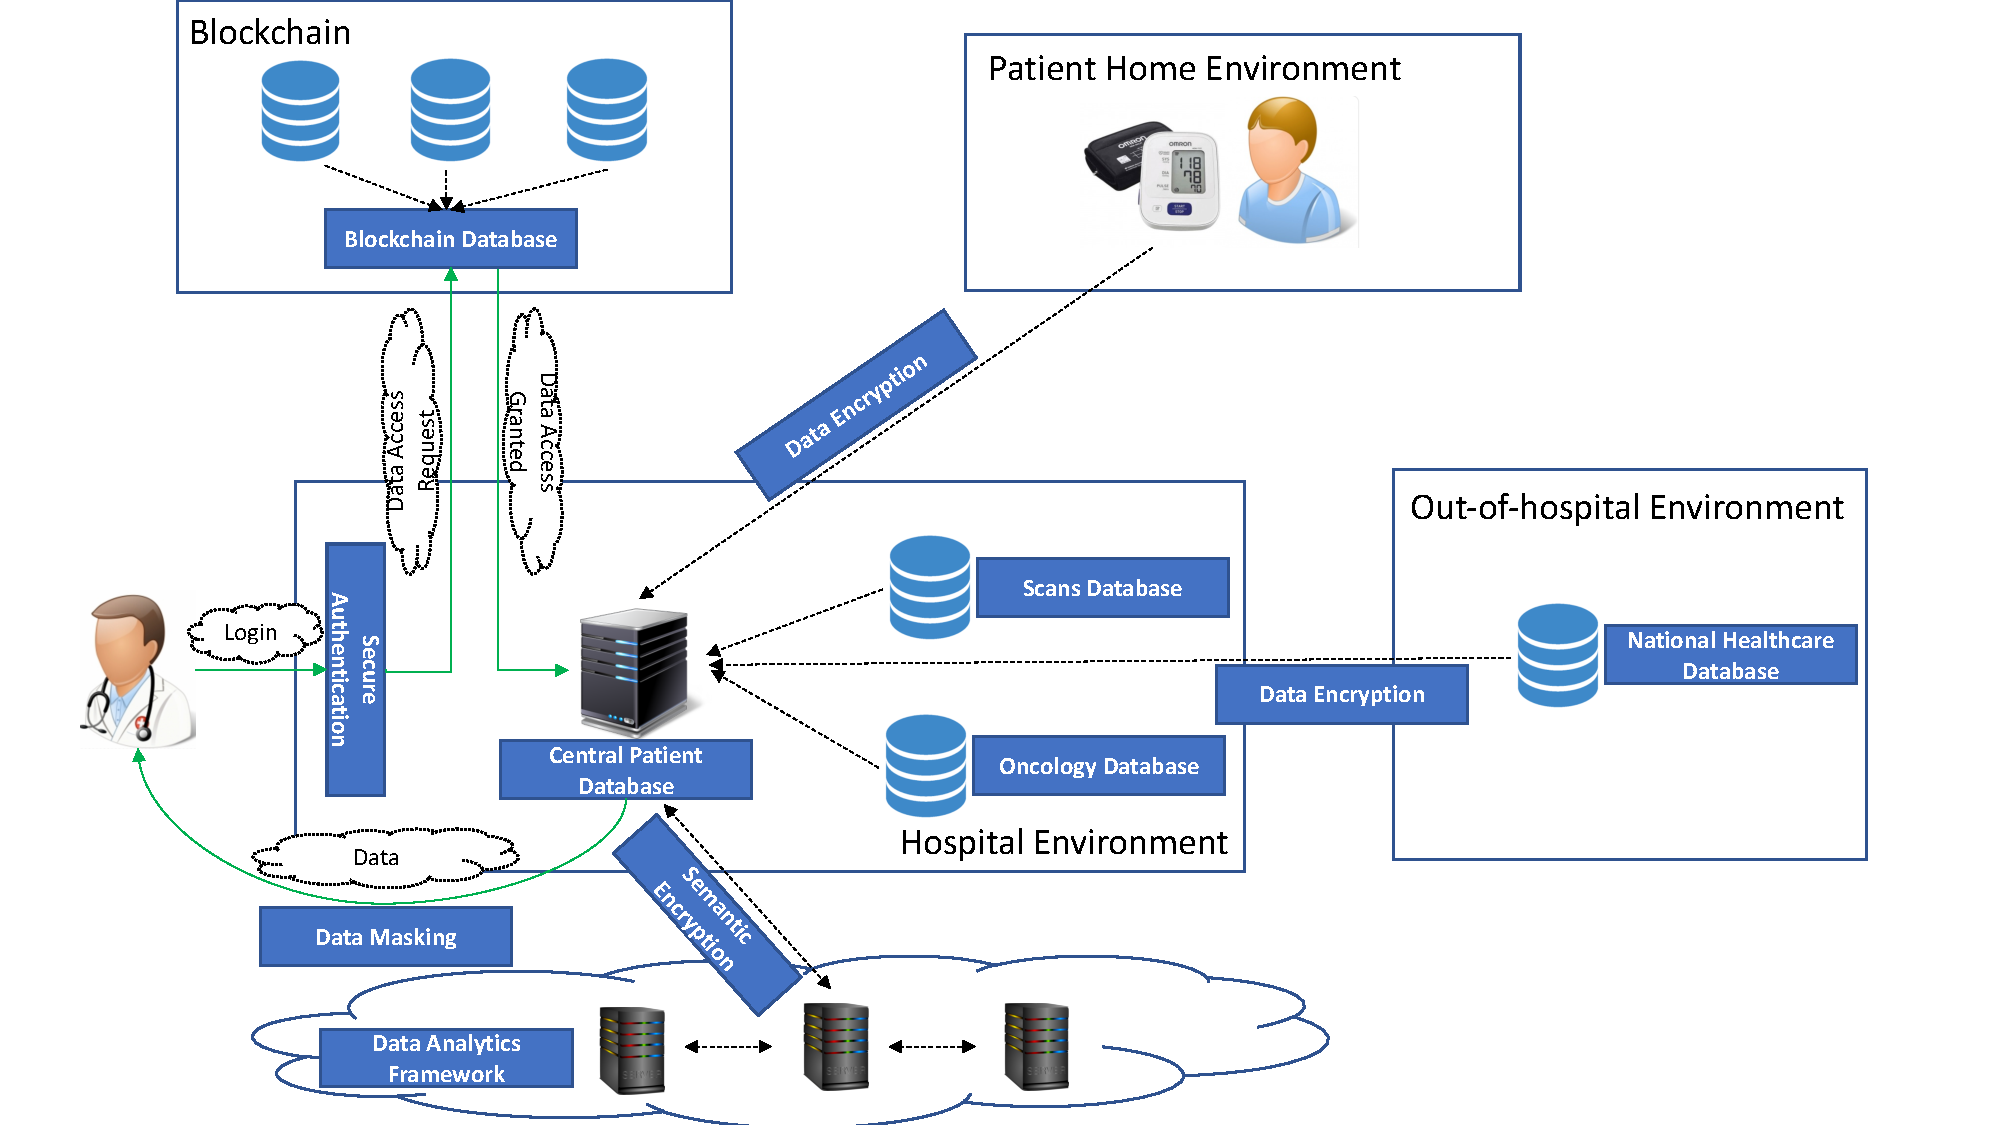
\includegraphics[width=90mm]{images/SerumsOverview.pdf}
    \caption{The overview of \emph{Serums} tool-chain}
    \label{fig:serumsTools}
\end{figure}

\noindent Figure~\ref{fig:serumsTools} gives an overview of the \emph{Serums} tool chain and the overall process of accessing and using the smart health centres that will be based on it. The core of it is the centralised data lake with various databases that forms the \emph{smart patient records} (see Section~\ref{sec:smartrecords}). These records contain all information about the patients, from static information such as date of birth, gender and contact information, to vital information such as weight, body mass index, allergies, to dynamic information about treatments and examinations. While we assume that all the records are stored in one location, the data that they refer to might reside in different distributed data storage technologies, i.e.~the records can contain \emph{remote pointers}. Some of the data for the records will be collected from within the healthcare system over trusted networks, while the other may be collected from the personal health monitoring devices from patient's home or workplace. The latter data may need to be sent over untrusted networks and, hence, needs to be secured using \emph{data masking and encryption} mechanisms.

For the purposes of developing and testing the complete infrastructure, it might be preferable to use \emph{synthetic} instead of real patient data, to avoid any privacy and security concerns. \emph{Data fabrication} (See Section~\ref{sec:datafabrication}) technology allows us to rapidly generate large volumes of the data that is the same in terms structure as the real data, but the fields of which are synthetically generated. The strict format of the smart patient records, with formally defined rules about the values of each field, relationships between different fields and well-formulated data interaction rules, allows this process to be performed automatically. 

The data is accessed using \emph{secure authentication} mechanisms (see Section~\ref{sec:authentication}). \textbf{VJ: Add a few sentence of why we need this and how it works}. As an additional layer of protection, a \emph{blockchain network} serves to control the access rights of the authorised agents to the patient records. Different agents will have different level of permissions, according to GDPR and other regulations. For example, the patient will have full access to its record, while any specialist will be able to access only the parts of the record that are relevant to the examination and diagnosis that they are to make. Insurers will have access to the medical history of the patient, but not to all the details about examinations and treatments. The blockchain will also be used to record the access history of the data. Note, however, that no actual data is stored in the blockchain - we only store access rules and transactions.

Once the user is authenticated and the access rights are verified, the requested data is sent to the user. This might involve \emph{masking} of the data, if parts of smart patient record need to be hidden from the user due to restricted access rights. The access transaction is also stored into the blockchain database.

Finally, different kinds of analysis will need to performed on patient data, for the diagnostic and treatment's predictions. Since the data in the patient records is distributed, the analytics will also need to be performed in distributed way. We need to make sure that no sensitive information is revealed by communicating this data between the central patient record database and the analytics model (which may reside, e.g., in the cloud). Additionally, we need to ensure that the analytics model itself does not accidentally leak any sensitive information. For this purpose, we are in the process of developing \emph{privacy-preserving distributed deep-learning analytics models} for data analysis (see Section~\ref{sec:dataanalysis}).

In the next section, we give more details about the individual tools of the toolchain.

%\section{Serums Technologies}

%\subsection{Smart Patient Records}
%\label{sec:smartrecords}


%\subsection{Data Fabrication}
%\label{sec:datafabrication}

%\subsection{Data Masking}
%\label{sec:datamasking}

%\subsection{Distributed Privacy-Preserving Data Analytics}
%\label{sec:dataanalysis}

%\subsection{Authentication and Authorisation}
%\label{sec:authentication}

%\subsection{Blockchain Smart Contracts}
%\label{sec:blockchain}



%\section{Evaluation}

%\subsection{Use Case Description}
%\label{usecase}





%\subsection*{Notes}

%Here are the items from the call for Healthcare Data and some comments/notes:
%\begin{enumerate}
%\item 
%\emph{Health data collection and analysis:}
%We have a lot of basis on this, we are clearly in both collection analytics.

%\item 
%\emph{Problems in health data processing:}
%We have some data processing aspects, so this is also strong for us.

%\item 
%\emph{Protection and security of personal health data:}
%We have this conceptually, and also concrete connections to GDPR.

%\item 
%\emph{Electronic health records and standards:}
%Exactly what we're doing for the first parts, standards not so clear?

%AV - suggest?

%COMMISSION RECOMMENDATION (EU) 2019/243 
%European Electronic Health Record exchange format 

%https://www.hl7.org/
%http://www.hl7.org/fhir/

%\end{enumerate}



